\documentclass{article}
\usepackage[english]{babel}
\usepackage[a4paper,top=2cm,bottom=2cm,left=3cm,right=3cm,marginparwidth=1.75cm]{geometry}
% Useful packages
\usepackage{color}%\textcolor;\color
\usepackage{amsmath}
\usepackage{graphicx}
\usepackage{caption}
\usepackage[colorlinks=true, allcolors=black]{hyperref}
\usepackage{pdfpages}
\usepackage{float}%图片包
%create figure in latex
\usepackage{tikz}
%\usepackage{cite}
\usepackage[backend=bibtex]{biblatex}
%more math symbols
\usepackage{amssymb}
%Information to be included in the title page:
\title{A fix method}
\author{Xin-Peng Li}
%Start of the document
\begin{document}
\maketitle
\section{A brief introduction}
We now confront a math problem when A is a complex number in \autoref{A}, and we must give a reasonable handling method.\\
Now we could think about another kind of heat-kernel-like regularization procedure, as shown below.
\begin{equation}
    \begin{split}
        \frac{1}{A}=&\frac{A^*}{AA^*}=\frac{A^*}{|A|^2}\\
        =&A^*\times \int_{0}^{+\infty}dx e^{-x|A|^2}\\
        =&\int_{0}^{+\infty}dxA^* e^{-x|A|^2}\\
        \rightarrow &\int_{\tau_{uv}^4}^{\tau_{ir}^4}dxA^* e^{-x|A|^2}
    \end{split}
\end{equation}
Notice that because of the dimension of $x$ is $GeV^{-4}$, we have to change the integral domain from $\tau^2$ to $\tau^4$.
\section{Model in zero temperature}
According to the derivative process of the contact interaction, we have already gotten the result of the gap equation in zero temperature.
\begin{equation}
    \begin{split}
        M=&m+M\frac{4}{3\pi}\frac{\alpha_{IR}}{m_G^2}\int_{0}^{\infty}ds s\frac{1}{s+M^2}\\
        \rightarrow&m+M\frac{4}{3\pi}\frac{\alpha_{IR}}{m_G^2}\int_{0}^{\infty}ds s\int_{\tau_{uv}^4}^{\tau_{ir}^4}dx(s+M^2)e^{-x(s+M^2)^2}\\
        =&m+M\frac{4}{3\pi}\frac{\alpha_{IR}}{m_G^2}\int_{\tau_{uv}^4}^{\tau_{ir}^4}dx\int_{0}^{\infty}ds s(s+M^2)e^{-x(s+M^2)^2}\\
        =&m+M\frac{4}{3\pi}\frac{\alpha_{IR}}{m_G^2}\int_{\tau_{uv}^4}^{\tau_{ir}^4}dx\frac{\sqrt{\pi}*Erfc[M^2\sqrt{x}]}{4x^{\frac{3}{2}}}\\
        =&m+M\frac{4}{3\pi}\frac{\alpha_{IR}}{m_G^2}[-\frac{\sqrt{\pi}*Erfc[M^2\sqrt{x}]}{2\sqrt{x}}-\frac{1}{2}M^2*ExpIntegralEi[-M^4x]]|_{x=\tau_{uv}^4}^{x=\tau_{ir}^4}
    \end{split}
\end{equation}
Because of the changing of the procedure of the heat-kernel-like regularization, we should slightly adjust the parameters to keep the result unchanged.\\
After calculation, we get the reasonable parameter: $\Lambda_{uv}=0.988$, and the result is shown below.
\begin{table}[H]
    \begin{center}
\begin{tabular}{|c|c|c|}
    \hline
    $m_u$ & $M_0$ & $M_u$ \\
    \hline
    0.007 GeV & 0.356 GeV&0.364 GeV \\
    \hline
\end{tabular}
\end{center}
\end{table}
\newpage
\section{Finite temperature and zero potential}
If $\mu=0$, we notice that $A^*=A$, so we obtain
\begin{equation}
    \begin{split}
        \mathcal{G} &=T\sum_{l=-\infty}^{+\infty}\int_{\tau_{uv}^4}^{\tau_{ir}^4}dx\int_{0}^{+\infty}ds s^{\frac{1}{2}}[s+M^2+\omega_l^2]e^{-x[s+M^2+\omega_l^2]^2}\\
        &=\frac{T}{4\sqrt{2}}\sum_{l=-\infty}^{+\infty}\int_{\tau_{uv}^4}^{\tau_{ir}^4}\frac{dx}{x}\sqrt{M^2+\omega_l^2}e^{-\frac{x}{2}[M^2+\omega_l^2]^2}*BesselK[\frac{1}{4},\frac{1}{2}[M^2+\omega_l^2]^2x]\\
        &\stackrel{t=\frac{1}{2}[M^2+\omega_l^2]^2x}{=}\frac{T}{4\sqrt{2}}\sum_{l=-\infty}^{+\infty}\sqrt{M^2+\omega_l^2}\int_{\frac{[M^2+\omega_l^2]^2}{2}\tau_{uv}^4}^{\frac{[M^2+\omega_l^2]^2}{2}\tau_{ir}^4}\frac{dt}{t}e^{-t}*BesselK[\frac{1}{4},t]\\
        &=\frac{T}{4\sqrt{2}}\sum_{l=-\infty}^{+\infty}\sqrt{M^2+\omega_l^2}f(t)|_{t=\frac{1}{2}[M^2+\omega_l^2]^2\tau_{uv}^4}^{t=\frac{1}{2}[M^2+\omega_l^2]^2\tau_{ir}^4}\\
        &=\frac{T}{2\sqrt{2}}\sum_{l=0}^{+\infty}\sqrt{M^2+\omega_l^2}f(t)|_{t=\frac{1}{2}[M^2+\omega_l^2]^2\tau_{uv}^4}^{t=\frac{1}{2}[M^2+\omega_l^2]^2\tau_{ir}^4}  ,
    \end{split}
\end{equation}
where
\begin{equation}
    \begin{split}
        f(t)&=\int\frac{dt}{t}e^{-t}*BesselK[\frac{1}{4},t]\\
        &=-\frac{2^{\frac{7}{4}}\pi*HypergeometricPFQ[\{-\frac{1}{4},\frac{1}{4}\},\{\frac{1}{2},\frac{3}{4}\},-2t]}{t^{\frac{1}{4}}*Gamma(\frac{3}{4})}\\
        &-\frac{2^{\frac{5}{4}}\pi t^{\frac{1}{4}}*HypergeometricPFQ[\{\frac{1}{4},\frac{3}{4}\},\{\frac{5}{4},\frac{3}{2}\},-2t]}{Gamma(\frac{5}{4})}
    \end{split}
\end{equation}
The function $f(t)$ is shown in the following figure.
\begin{figure}[!htb]
    \centering
    \includegraphics[width=0.5\linewidth]{pic/trend.jpg}
    \caption{$f(t)$ and t from 0 to 1.}
\end{figure}
\\From the figure, We could find that $\mathcal{G}$ must be converge.\\
Next, we need to deal with the sum of l. This is a troublesome thing, because we can not calculate it analytically. So we need to think about a numerical computation method.\\
Just to give a trend, we could calculate the result $\mathcal{G}$ varyies with l, i.e., 
\begin{equation}
    \mathcal{G}(l_0)=\frac{T}{2\sqrt{2}}\sum_{l=0}^{l_0}\sqrt{M^2+\omega_l^2}f(t)|_{t=\frac{1}{2}[M^2+\omega_l^2]^2\tau_{uv}^4}^{t=\frac{1}{2}[M^2+\omega_l^2]^2\tau_{ir}^4}= \frac{T}{2\sqrt{2}}\sum_{l=0}^{l_0}g_l,
\end{equation}
And we could get the following chart. 
\begin{table}[H]
\begin{minipage}{0.45\textwidth}
\begin{center}
    \begin{tabular}{|c|c|c|}
    \hline
    $l_0$ &$ g_{l_0} $& Sum of $g_l$\\
    \hline
    0 &$ 7.5732657 $ &7.5732657\\
    \hline
    1 &$  6.7753596 $ &14.3486253\\
    \hline
    2 &$  5.2454196 $ &19.5940449\\
    \hline
    3 &$   3.7281628 $ &23.3222077\\
    \hline
    4 &$   2.4768575 $ &25.7990652\\
    \hline
    \end{tabular}
    \caption{$T=0.02$ and $M=0.02$}
\end{center}
\end{minipage}
\begin{minipage}{0.45\textwidth}
    \begin{center}
        \begin{tabular}{|c|c|c|}
        \hline
        $l_0$ &$ g_{l_0} $& Sum of $g_l$\\
        \hline
        0 &$ 1.7293313 $ &1.7293313\\
        \hline
        1 &$  7.87*10^{-8} $ &1.7293314\\
        \hline
        2 &$  0 $ &1.7293314\\
        \hline
        3 &$   0 $ &1.7293314\\
        \hline
        4 &$   0 $ &1.7293314\\
        \hline
        \end{tabular}
        \caption{$T=0.2$ and $M=0.2$}
    \end{center}
    \end{minipage}
\end{table}
The table shows that the influential range of $l$ is depend on the value of T and M.\\
So we add a judge procedure, i.e., we stop the sum of $l$ when the contributions of the $l$ term are less than 0.001 times the $l=0$ term.\\
The remaining procedure is just calculating $M$ at every $T$, and we could get the final results.
    \begin{figure}[H]
    \centering
    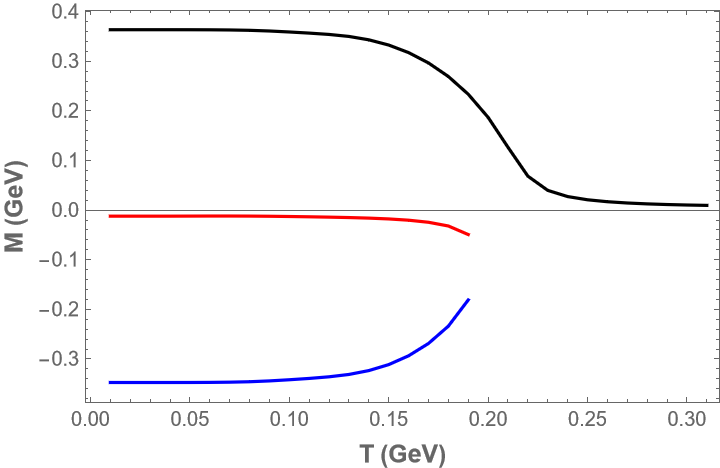
\includegraphics[width=0.7\linewidth]{pic/M-T.png}
    \caption{$\mu=0$ and T from 0 to 0.3 GeV.}
    \end{figure}
\newpage
\section{Finite temperature and chemical potential}
If $\mu\neq0$, we obtain the following equation.
\begin{equation}
    \begin{split}
        \mathcal{G} &=T\sum_{l=-\infty}^{+\infty}\int_{\tau_{uv}^4}^{\tau_{ir}^4}dx\int_{0}^{+\infty}ds s^{\frac{1}{2}}[s+M^2+\widetilde{\omega_l}^2]^*e^{-x|s+M^2+\widetilde{\omega_l}^2|^2}\\
        &=T\sum_{l=-\infty}^{+\infty}\int_{\tau_{uv}^4}^{\tau_{ir}^4}dx\int_{0}^{+\infty}ds s^{\frac{1}{2}}(s+M^2+\omega_l^2-\mu^2-2I\omega_l\mu)e^{-x[(s+M^2+\omega_l^2-\mu^2)^2+(2\omega_l\mu)^2]}\\
        &=\frac{T}{4\sqrt{2}}\sum_{l=-\infty}^{+\infty}\sqrt{M^2+\omega_l^2-\mu^2}\int_{\tau_{uv}^4}^{\tau_{ir}^4}
        \frac{dx}{x}e^{-\frac{1}{2}((M^2+\omega_l^2)^2-2(M^2-3\omega_l^2)\mu^2+\mu^4)x}\\
        &((1+4I\omega_l\mu(M^2+\omega_l^2-\mu^2)x)BesselK[\frac{1}{4},\frac{1}{2}(M^2+\omega_l^2-\mu^2)^2x]\\
        &-4I\omega_l\mu(M^2+\omega_l^2-\mu^2)x BesselK[\frac{3}{4},\frac{1}{2}(M^2+\omega_l^2-\mu^2)^2x])\\
        &\stackrel{t=\frac{1}{2}(M^2+\omega_l^2-\mu^2)^2x}{=}\frac{T}{4\sqrt{2}}\sum_{l=-\infty}^{+\infty}\sqrt{M^2+\omega_l^2-\mu^2}\int_{\frac{[M^2+\omega_l^2-\mu^2]^2}{2}\tau_{uv}^4}^{\frac{[M^2+\omega_l^2-\mu^2]^2}{2}\tau_{ir}^4}\frac{dt}{t}e^{-\frac{(M^2+\omega_l^2)^2-2(M^2-3\omega_l^2)\mu^2+\mu^4}{(M^2+\omega_l^2-\mu^2)^2}t}\\
        &((1+\frac{8I\omega_l\mu}{M^2+\omega_l^2-\mu^2}t)BesselK[\frac{1}{4},t]-\frac{8I\omega_l\mu}{M^2+\omega_l^2-\mu^2}t BesselK[\frac{3}{4},t])\\
        &=\frac{T}{4\sqrt{2}}\sum_{l=-\infty}^{+\infty}\sqrt{M^2+\omega_l^2-\mu^2}\int_{\frac{[M^2+\omega_l^2-\mu^2]^2}{2}\tau_{uv}^4}^{\frac{[M^2+\omega_l^2-\mu^2]^2}{2}\tau_{ir}^4}\frac{dt}{t}e^{-(1+\beta^2)t}\\
        &((1+2\sqrt{2}I\beta t)BesselK[\frac{1}{4},t]-2\sqrt{2}I\beta t BesselK[\frac{3}{4},t]),
    \end{split}
\end{equation}
where
\begin{equation}
    \beta=\frac{2\sqrt{2}\omega_l\mu}{M^2+\omega_l^2-\mu^2}.
\end{equation}
We could not find the primitive function of the integrand. However, we could calculate the result numerically, and we could imagine that we need to cut off $l$ at a certain value which depends on the parameters. The judge procedure is the same as before, just use the absolute value of the complex number.\\
We get the final results as below.
    \begin{figure}[H]
    \centering
    \includegraphics[width=0.7\linewidth]{pic/M-μ.png}
    \caption{$T=0.0005$ and $\mu$ from 0 to 0.5 GeV.}
    \end{figure}
\newpage
\section{Some notes}
\begin{itemize}
    \item The trend seems nice in finite temperature and potential. Especially in finite potential, the result shows the first-order phase transformations.
    \item The flaw is that the quark mass will increase with the potential, this feature maybe caused by the higher power in the regularization.
\end{itemize}
\end{document}

